\PassOptionsToPackage{unicode=true}{hyperref} % options for packages loaded elsewhere
\PassOptionsToPackage{hyphens}{url}
%
\documentclass[]{article}
\usepackage{lmodern}
\usepackage{amssymb,amsmath}
\usepackage{ifxetex,ifluatex}
\usepackage{fixltx2e} % provides \textsubscript
\ifnum 0\ifxetex 1\fi\ifluatex 1\fi=0 % if pdftex
  \usepackage[T1]{fontenc}
  \usepackage[utf8]{inputenc}
  \usepackage{textcomp} % provides euro and other symbols
\else % if luatex or xelatex
  \usepackage{unicode-math}
  \defaultfontfeatures{Ligatures=TeX,Scale=MatchLowercase}
\fi
% use upquote if available, for straight quotes in verbatim environments
\IfFileExists{upquote.sty}{\usepackage{upquote}}{}
% use microtype if available
\IfFileExists{microtype.sty}{%
\usepackage[]{microtype}
\UseMicrotypeSet[protrusion]{basicmath} % disable protrusion for tt fonts
}{}
\IfFileExists{parskip.sty}{%
\usepackage{parskip}
}{% else
\setlength{\parindent}{0pt}
\setlength{\parskip}{6pt plus 2pt minus 1pt}
}
\usepackage{hyperref}
\hypersetup{
            pdftitle={Muscle Tsc1 Knockout Food Preference Test},
            pdfauthor={Detrick Snyder and Dave Bridges},
            pdfborder={0 0 0},
            breaklinks=true}
\urlstyle{same}  % don't use monospace font for urls
\usepackage[margin=1in]{geometry}
\usepackage{color}
\usepackage{fancyvrb}
\newcommand{\VerbBar}{|}
\newcommand{\VERB}{\Verb[commandchars=\\\{\}]}
\DefineVerbatimEnvironment{Highlighting}{Verbatim}{commandchars=\\\{\}}
% Add ',fontsize=\small' for more characters per line
\usepackage{framed}
\definecolor{shadecolor}{RGB}{248,248,248}
\newenvironment{Shaded}{\begin{snugshade}}{\end{snugshade}}
\newcommand{\AlertTok}[1]{\textcolor[rgb]{0.94,0.16,0.16}{#1}}
\newcommand{\AnnotationTok}[1]{\textcolor[rgb]{0.56,0.35,0.01}{\textbf{\textit{#1}}}}
\newcommand{\AttributeTok}[1]{\textcolor[rgb]{0.77,0.63,0.00}{#1}}
\newcommand{\BaseNTok}[1]{\textcolor[rgb]{0.00,0.00,0.81}{#1}}
\newcommand{\BuiltInTok}[1]{#1}
\newcommand{\CharTok}[1]{\textcolor[rgb]{0.31,0.60,0.02}{#1}}
\newcommand{\CommentTok}[1]{\textcolor[rgb]{0.56,0.35,0.01}{\textit{#1}}}
\newcommand{\CommentVarTok}[1]{\textcolor[rgb]{0.56,0.35,0.01}{\textbf{\textit{#1}}}}
\newcommand{\ConstantTok}[1]{\textcolor[rgb]{0.00,0.00,0.00}{#1}}
\newcommand{\ControlFlowTok}[1]{\textcolor[rgb]{0.13,0.29,0.53}{\textbf{#1}}}
\newcommand{\DataTypeTok}[1]{\textcolor[rgb]{0.13,0.29,0.53}{#1}}
\newcommand{\DecValTok}[1]{\textcolor[rgb]{0.00,0.00,0.81}{#1}}
\newcommand{\DocumentationTok}[1]{\textcolor[rgb]{0.56,0.35,0.01}{\textbf{\textit{#1}}}}
\newcommand{\ErrorTok}[1]{\textcolor[rgb]{0.64,0.00,0.00}{\textbf{#1}}}
\newcommand{\ExtensionTok}[1]{#1}
\newcommand{\FloatTok}[1]{\textcolor[rgb]{0.00,0.00,0.81}{#1}}
\newcommand{\FunctionTok}[1]{\textcolor[rgb]{0.00,0.00,0.00}{#1}}
\newcommand{\ImportTok}[1]{#1}
\newcommand{\InformationTok}[1]{\textcolor[rgb]{0.56,0.35,0.01}{\textbf{\textit{#1}}}}
\newcommand{\KeywordTok}[1]{\textcolor[rgb]{0.13,0.29,0.53}{\textbf{#1}}}
\newcommand{\NormalTok}[1]{#1}
\newcommand{\OperatorTok}[1]{\textcolor[rgb]{0.81,0.36,0.00}{\textbf{#1}}}
\newcommand{\OtherTok}[1]{\textcolor[rgb]{0.56,0.35,0.01}{#1}}
\newcommand{\PreprocessorTok}[1]{\textcolor[rgb]{0.56,0.35,0.01}{\textit{#1}}}
\newcommand{\RegionMarkerTok}[1]{#1}
\newcommand{\SpecialCharTok}[1]{\textcolor[rgb]{0.00,0.00,0.00}{#1}}
\newcommand{\SpecialStringTok}[1]{\textcolor[rgb]{0.31,0.60,0.02}{#1}}
\newcommand{\StringTok}[1]{\textcolor[rgb]{0.31,0.60,0.02}{#1}}
\newcommand{\VariableTok}[1]{\textcolor[rgb]{0.00,0.00,0.00}{#1}}
\newcommand{\VerbatimStringTok}[1]{\textcolor[rgb]{0.31,0.60,0.02}{#1}}
\newcommand{\WarningTok}[1]{\textcolor[rgb]{0.56,0.35,0.01}{\textbf{\textit{#1}}}}
\usepackage{longtable,booktabs}
% Fix footnotes in tables (requires footnote package)
\IfFileExists{footnote.sty}{\usepackage{footnote}\makesavenoteenv{longtable}}{}
\usepackage{graphicx,grffile}
\makeatletter
\def\maxwidth{\ifdim\Gin@nat@width>\linewidth\linewidth\else\Gin@nat@width\fi}
\def\maxheight{\ifdim\Gin@nat@height>\textheight\textheight\else\Gin@nat@height\fi}
\makeatother
% Scale images if necessary, so that they will not overflow the page
% margins by default, and it is still possible to overwrite the defaults
% using explicit options in \includegraphics[width, height, ...]{}
\setkeys{Gin}{width=\maxwidth,height=\maxheight,keepaspectratio}
\setlength{\emergencystretch}{3em}  % prevent overfull lines
\providecommand{\tightlist}{%
  \setlength{\itemsep}{0pt}\setlength{\parskip}{0pt}}
\setcounter{secnumdepth}{5}
% Redefines (sub)paragraphs to behave more like sections
\ifx\paragraph\undefined\else
\let\oldparagraph\paragraph
\renewcommand{\paragraph}[1]{\oldparagraph{#1}\mbox{}}
\fi
\ifx\subparagraph\undefined\else
\let\oldsubparagraph\subparagraph
\renewcommand{\subparagraph}[1]{\oldsubparagraph{#1}\mbox{}}
\fi

% set default figure placement to htbp
\makeatletter
\def\fps@figure{htbp}
\makeatother


\title{Muscle Tsc1 Knockout Food Preference Test}
\author{Detrick Snyder and Dave Bridges}
\date{January 2, 2018}

\begin{document}
\maketitle

{
\setcounter{tocdepth}{2}
\tableofcontents
}
These data can be found in
\textbf{/Users/davebrid/Documents/GitHub/TissueSpecificTscKnockouts/Mouse
Data/Muscle Tsc1 Knockout} in a file named \textbf{mTSC Macronutrient
Preference.csv}. This script was most recently updated on \textbf{Fri
Mar 27 09:52:58 2020}.

\hypertarget{analysis}{%
\section{Analysis}\label{analysis}}

\begin{longtable}[]{@{}llr@{}}
\caption{Animals enrolled in this study}\tabularnewline
\toprule
Sex & Genotype & n\tabularnewline
\midrule
\endfirsthead
\toprule
Sex & Genotype & n\tabularnewline
\midrule
\endhead
M & fl/fl;+/+ & 6\tabularnewline
M & fl/fl;tg/+ & 9\tabularnewline
F & fl/fl;+/+ & 11\tabularnewline
F & fl/fl;tg/+ & 9\tabularnewline
\bottomrule
\end{longtable}

\begin{longtable}[]{@{}rllrrrrr@{}}
\caption{Calculated data for each cage.}\tabularnewline
\toprule
ear.tag & Sex & Genotype & KDC & KD & Total & KD.Pref &
KD.Pct\tabularnewline
\midrule
\endfirsthead
\toprule
ear.tag & Sex & Genotype & KDC & KD & Total & KD.Pref &
KD.Pct\tabularnewline
\midrule
\endhead
7454 & M & fl/fl;+/+ & 0.2 & 2.2 & 2.4 & 11.000 & 91.7\tabularnewline
7461 & M & fl/fl;+/+ & 0.1 & 1.9 & 2.0 & 19.000 & 95.0\tabularnewline
7462 & M & fl/fl;+/+ & 0.1 & 2.1 & 2.2 & 21.000 & 95.5\tabularnewline
7766 & M & fl/fl;+/+ & 6.4 & 4.8 & 11.2 & 0.750 & 42.9\tabularnewline
7928 & M & fl/fl;+/+ & 0.9 & 7.4 & 8.3 & 8.222 & 89.2\tabularnewline
7929 & M & fl/fl;+/+ & 0.4 & 4.1 & 4.5 & 10.250 & 91.1\tabularnewline
7428 & F & fl/fl;+/+ & 0.6 & 6.6 & 7.2 & 11.000 & 91.7\tabularnewline
7429 & F & fl/fl;+/+ & 0.5 & 7.6 & 8.1 & 15.200 & 93.8\tabularnewline
7431 & F & fl/fl;+/+ & 3.6 & 4.8 & 8.4 & 1.333 & 57.1\tabularnewline
7896 & F & fl/fl;+/+ & 8.6 & 4.2 & 12.8 & 0.488 & 32.8\tabularnewline
7931 & F & fl/fl;+/+ & 7.0 & 6.4 & 13.4 & 0.914 & 47.8\tabularnewline
7932 & F & fl/fl;+/+ & 5.4 & 6.9 & 12.3 & 1.278 & 56.1\tabularnewline
8336 & F & fl/fl;+/+ & -1.1 & 6.0 & 4.9 & -5.455 & 122.4\tabularnewline
8337 & F & fl/fl;+/+ & 2.4 & 5.7 & 8.1 & 2.375 & 70.4\tabularnewline
8338 & F & fl/fl;+/+ & -0.8 & 5.9 & 5.1 & -7.375 & 115.7\tabularnewline
8339 & F & fl/fl;+/+ & 7.5 & 5.5 & 13.0 & 0.733 & 42.3\tabularnewline
8379 & F & fl/fl;+/+ & 8.6 & 4.6 & 13.2 & 0.535 & 34.8\tabularnewline
7425 & M & fl/fl;tg/+ & NA & 3.1 & NA & NA & NA\tabularnewline
7426 & M & fl/fl;tg/+ & 7.5 & 2.7 & 10.2 & 0.360 & 26.5\tabularnewline
7427 & M & fl/fl;tg/+ & 1.5 & 9.1 & 10.6 & 6.067 & 85.8\tabularnewline
7455 & M & fl/fl;tg/+ & NA & 0.1 & NA & NA & NA\tabularnewline
7456 & M & fl/fl;tg/+ & 0.5 & 2.7 & 3.2 & 5.400 & 84.4\tabularnewline
7555 & M & fl/fl;tg/+ & 3.3 & NA & NA & NA & NA\tabularnewline
7893 & M & fl/fl;tg/+ & 3.7 & 8.3 & 12.0 & 2.243 & 69.2\tabularnewline
7894 & M & fl/fl;tg/+ & 6.5 & 6.5 & 13.0 & 1.000 & 50.0\tabularnewline
7927 & M & fl/fl;tg/+ & 6.6 & 2.4 & 9.0 & 0.364 & 26.7\tabularnewline
7457 & F & fl/fl;tg/+ & 0.9 & 2.8 & 3.7 & 3.111 & 75.7\tabularnewline
7460 & F & fl/fl;tg/+ & 2.3 & 1.2 & 3.5 & 0.522 & 34.3\tabularnewline
7464 & F & fl/fl;tg/+ & 0.4 & 1.6 & 2.0 & 4.000 & 80.0\tabularnewline
7466 & F & fl/fl;tg/+ & 1.2 & 2.4 & 3.6 & 2.000 & 66.7\tabularnewline
7467 & F & fl/fl;tg/+ & 0.4 & 2.3 & 2.7 & 5.750 & 85.2\tabularnewline
7897 & F & fl/fl;tg/+ & 1.9 & 8.1 & 10.0 & 4.263 & 81.0\tabularnewline
7898 & F & fl/fl;tg/+ & 17.5 & 6.3 & 23.8 & 0.360 & 26.5\tabularnewline
7899 & F & fl/fl;tg/+ & 14.1 & 7.5 & 21.6 & 0.532 & 34.7\tabularnewline
8380 & F & fl/fl;tg/+ & 23.7 & 4.2 & 27.9 & 0.177 & 15.1\tabularnewline
\bottomrule
\end{longtable}

\begin{longtable}[]{@{}llrrrrrr@{}}
\toprule
Sex & Genotype & Preference & Preference.Error & PReference.SD & Percent
& Percent.Error & N\tabularnewline
\midrule
\endhead
M & fl/fl;+/+ & 11.70 & 3.024 & 7.41 & 84.2 & 8.33 & 6\tabularnewline
M & fl/fl;tg/+ & 2.57 & 0.851 & NA & 57.1 & 8.98 & 9\tabularnewline
F & fl/fl;+/+ & 1.91 & 1.923 & 6.38 & 69.5 & 9.59 & 11\tabularnewline
F & fl/fl;tg/+ & 2.30 & 0.687 & 2.06 & 55.5 & 9.15 & 9\tabularnewline
\bottomrule
\end{longtable}

\hypertarget{statistics}{%
\subsection{Statistics}\label{statistics}}

\begin{longtable}[]{@{}lrrrr@{}}
\caption{Genotype and Sex Dependent Effects on Relative
Preference.}\tabularnewline
\toprule
term & estimate & std.error & statistic & p.value\tabularnewline
\midrule
\endfirsthead
\toprule
term & estimate & std.error & statistic & p.value\tabularnewline
\midrule
\endhead
(Intercept) & 8.74 & 1.91 & 4.59 & 0.000\tabularnewline
SexF & -5.21 & 2.06 & -2.54 & 0.017\tabularnewline
Genotypefl/fl;tg/+ & -3.20 & 2.00 & -1.61 & 0.119\tabularnewline
\bottomrule
\end{longtable}

\begin{longtable}[]{@{}lrrrr@{}}
\caption{Genotype and Sex Dependent Effects on Relative Preference.
Model with moderating effect of sex on genotype.}\tabularnewline
\toprule
term & estimate & std.error & statistic & p.value\tabularnewline
\midrule
\endfirsthead
\toprule
term & estimate & std.error & statistic & p.value\tabularnewline
\midrule
\endhead
(Intercept) & 11.70 & 2.11 & 5.55 & 0.000\tabularnewline
SexF & -9.79 & 2.62 & -3.73 & 0.001\tabularnewline
Genotypefl/fl;tg/+ & -9.13 & 2.98 & -3.06 & 0.005\tabularnewline
SexF:Genotypefl/fl;tg/+ & 9.52 & 3.78 & 2.52 & 0.018\tabularnewline
\bottomrule
\end{longtable}

\begin{longtable}[]{@{}lrrrr@{}}
\caption{Sex Dependent Effects on Relative Preference, wild-type
only.}\tabularnewline
\toprule
term & estimate & std.error & statistic & p.value\tabularnewline
\midrule
\endfirsthead
\toprule
term & estimate & std.error & statistic & p.value\tabularnewline
\midrule
\endhead
(Intercept) & 11.70 & 2.75 & 4.25 & 0.001\tabularnewline
SexF & -9.79 & 3.42 & -2.86 & 0.012\tabularnewline
\bottomrule
\end{longtable}

\hypertarget{boxplots}{%
\subsection{Boxplots}\label{boxplots}}

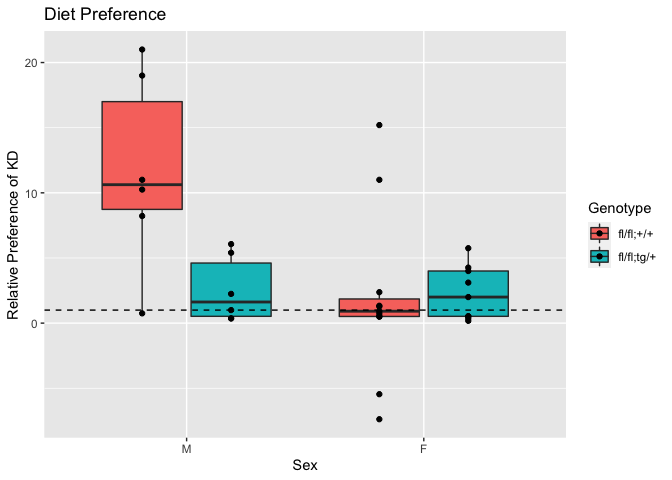
\includegraphics{figures/knockout-effects-boxplot-1.png}

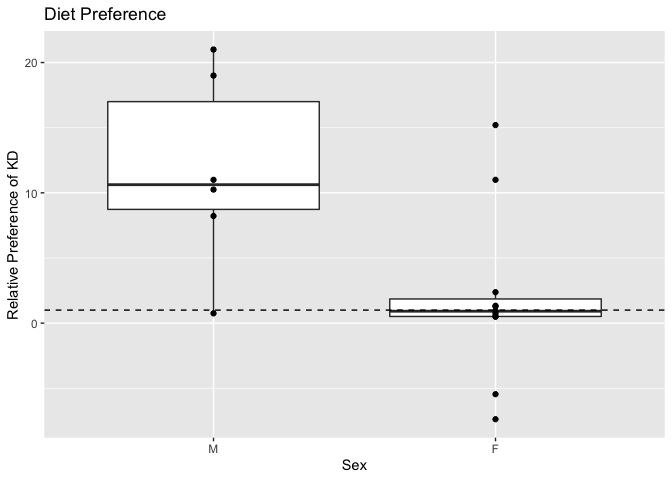
\includegraphics{figures/sex-effects-boxplot-1.png}

\hypertarget{barplots}{%
\subsection{Barplots}\label{barplots}}

\begin{figure}
\centering
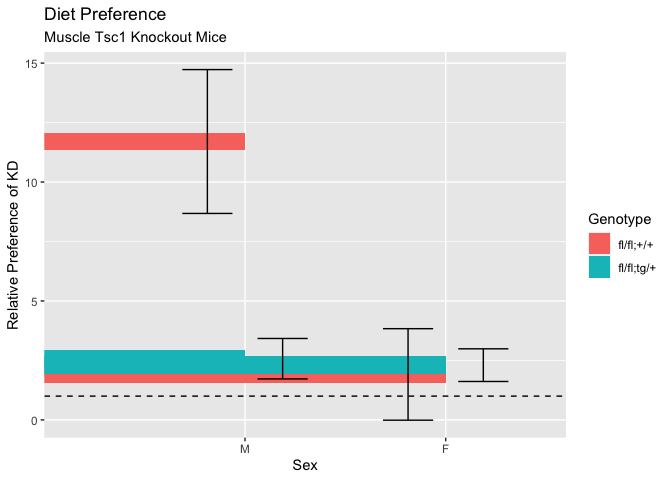
\includegraphics{figures/knockout-effects-barplot-relative-preference-1.png}
\caption{Effects of genotype on macronutrient preference}
\end{figure}

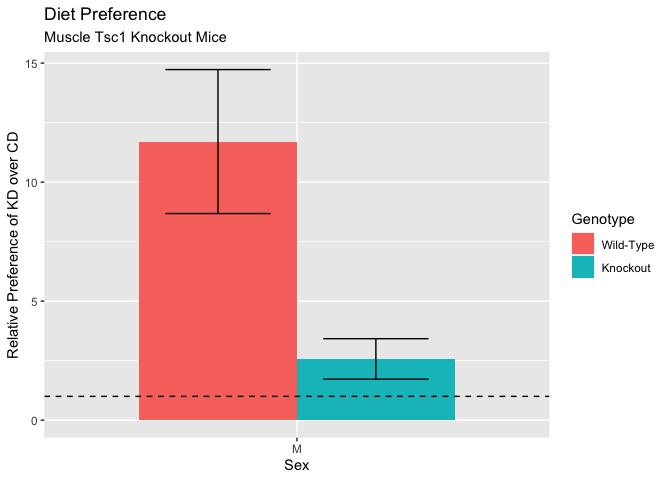
\includegraphics{figures/knockout-effects-barplot-relative-preference-males-1.png}
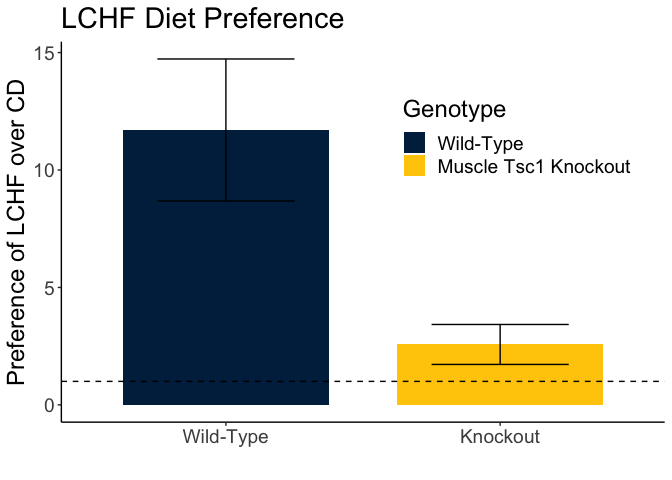
\includegraphics{figures/knockout-effects-barplot-relative-preference-males-2.png}
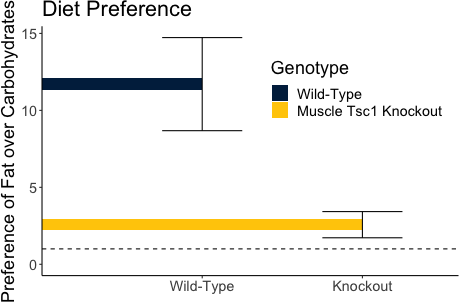
\includegraphics{figures/knockout-effects-barplot-relative-preference-males-3.png}

\begin{figure}
\centering
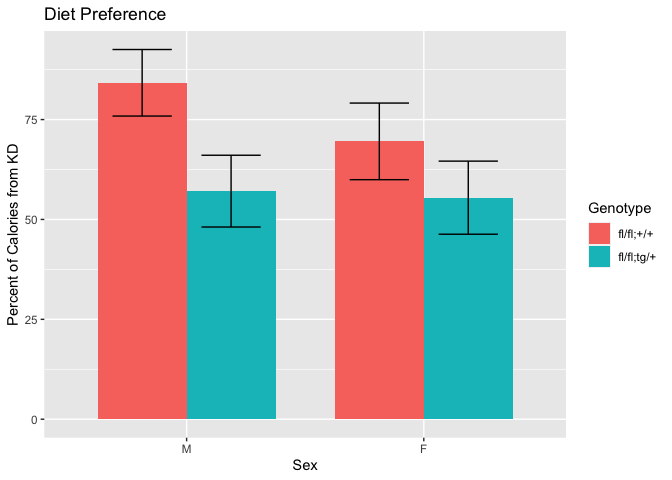
\includegraphics{figures/knockout-effects-barplot-percent-1.png}
\caption{Effects of genotype on macronutrient percent of calories from
KD}
\end{figure}

\begin{figure}
\centering
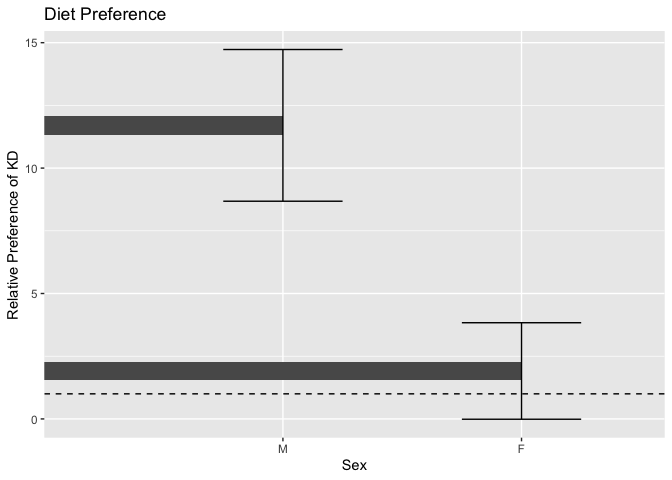
\includegraphics{figures/sex-effects-barplot-1.png}
\caption{Effects of sex on macronutrient preference}
\end{figure}

\hypertarget{interpretation}{%
\section{Interpretation}\label{interpretation}}

There is a preference towards ketogenic diet over its control diet.

\hypertarget{session-information}{%
\section{Session Information}\label{session-information}}

\begin{Shaded}
\begin{Highlighting}[]
\KeywordTok{sessionInfo}\NormalTok{()}
\end{Highlighting}
\end{Shaded}

\begin{verbatim}
## R version 3.6.3 (2020-02-29)
## Platform: x86_64-apple-darwin15.6.0 (64-bit)
## Running under: macOS Catalina 10.15.3
## 
## Matrix products: default
## BLAS:   /Library/Frameworks/R.framework/Versions/3.6/Resources/lib/libRblas.0.dylib
## LAPACK: /Library/Frameworks/R.framework/Versions/3.6/Resources/lib/libRlapack.dylib
## 
## locale:
## [1] en_US.UTF-8/en_US.UTF-8/en_US.UTF-8/C/en_US.UTF-8/en_US.UTF-8
## 
## attached base packages:
## [1] stats     graphics  grDevices utils     datasets  methods   base     
## 
## other attached packages:
## [1] forcats_0.5.0      ggplot2_3.3.0.9000 broom_0.5.5        readr_1.3.1       
## [5] dplyr_0.8.5        tidyr_1.0.2        knitr_1.28        
## 
## loaded via a namespace (and not attached):
##  [1] Rcpp_1.0.4       pillar_1.4.3     compiler_3.6.3   highr_0.8       
##  [5] tools_3.6.3      digest_0.6.25    evaluate_0.14    lifecycle_0.2.0 
##  [9] tibble_2.1.3     nlme_3.1-144     gtable_0.3.0     lattice_0.20-38 
## [13] pkgconfig_2.0.3  rlang_0.4.5      magick_2.3       yaml_2.2.1      
## [17] xfun_0.12        withr_2.1.2      stringr_1.4.0    generics_0.0.2  
## [21] vctrs_0.2.4      hms_0.5.3        grid_3.6.3       tidyselect_1.0.0
## [25] glue_1.3.2       R6_2.4.1         rmarkdown_2.1    farver_2.0.3    
## [29] purrr_0.3.3      magrittr_1.5     backports_1.1.5  scales_1.1.0    
## [33] htmltools_0.4.0  assertthat_0.2.1 colorspace_1.4-1 labeling_0.3    
## [37] stringi_1.4.6    munsell_0.5.0    crayon_1.3.4
\end{verbatim}

\end{document}
